\documentclass[12pt]{article}

\usepackage[english]{babel}
\usepackage[utf8]{inputenc}
\usepackage[T1]{fontenc}
\usepackage{graphicx}
\usepackage{amsmath}
\usepackage{fancyhdr}
\usepackage{siunitx}
\usepackage{listings}

\makeatletter
\def\@seccntformat#1{\csname the#1\endcsname\hspace*{0.5em}$|$\hspace*{0.5em}}
\makeatother

\pagestyle{fancy}

\title{\textbf{Quartz resonator} \\ SCI-C0200}
\author{Joonatan Bergholm 507260 \\ Osama Abuzaid XXXXXX}

\begin{document}

\pagenumbering{gobble}
\maketitle
\newpage

\pagenumbering{arabic}

\tableofcontents
\newpage

\section{Introduction}

In this assignment we investigated electronic properties of one of the most common electronic components, the quartz tuning fork or quartz resonator, like one in figure \ref{fig:kvres}. It is used in watches and other every day electrical appliances to provide a stable clocking frequency. Typically the frequency is $f_0 = \SI{32768}{\hertz}$, because is is a round number ($32768_{10} = {2^{15}}_{10} = 1000000000000000_2$) in base 2, which is commonly used in electrical appliances.

Contrary to conventional tuning fork, one does not need generate mechanical excitation
on the quartz tuning fork, because quartz has piezoelectric properties and thus mechanical excitation can be replaced with electronic one.

\section{Theory}

\begin{figure}
	\centering
	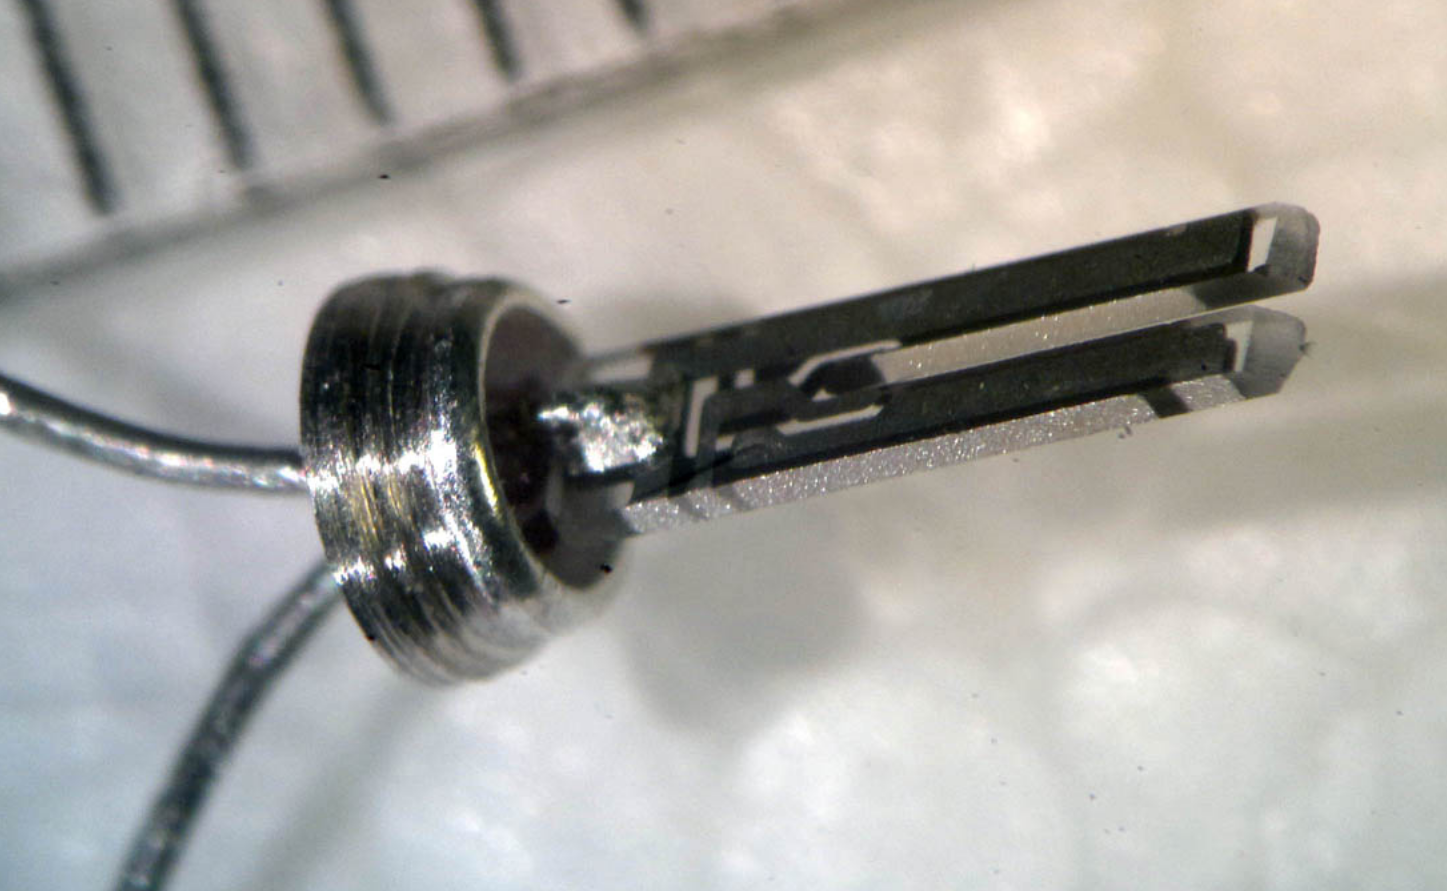
\includegraphics[width = \textwidth]{kuvat/kvres.png}
	\caption{Quartz resonator}
	\label{fig:kvres}
\end{figure}

\section{Results}

\begin{figure}
	\centering
	\includegraphics[width = \textwidth]{kuvat/steadystate.png}
	\caption{Steady state}
	\label{fig:steady}
\end{figure}

\appendix

\section{Source code}

\lstinputlisting[caption = ac.m]{matlab/ac.m}
%\lstinputlisting[caption = ac.m]{matlab/DAQreadout.m}

\section{Pretasks}

\subsection{Session 1}

\subsubsection{Task 1}

In this project we are supposed to study electric properties of quartz resonators and build a circuit, which is used to collect data from the resonator. Data is then analyzed with MATLAB. Also we are going to measure some properties of the circuit itself.

\subsubsection{Task 2}

$V_+$ is connected to ground, so $V_+ = 0$.

\begin{align*}
V_{out} =& A(V_+ - V_-) \\
\Rightarrow V_{out} =& -AV_-
\end{align*}

Then according to Kirchoff II and Ohm's law,

\begin{align*}
V_- - V_{out} = R_f I \quad \wedge & \quad I = \frac{V_{in} - V_{out}}{R_f + R_{in}} \\
\Rightarrow V_- =& R_f \frac{V_{in} - V_{out}}{R_f + R_{in}} + V_{out} \\
\Rightarrow V_- =& \frac{R_f V_{in} - R_f V_{out}}{R_f + R_{in}} + \frac{R_f V_{out} + R_{in} V_{out}}{R_f + R_{in}} \\
\Rightarrow V_- &= \frac{R_f V_{in} + R_{in} V_{out}}{R_f + R_{in}} \\
\end{align*}

Then combining these two equations, we obtain $V_{out}$ as function of $V_{in}$.

\begin{align*}
V_{out} &= -A\frac{R_f V_{in} + R_{in} V_{out}}{R_f + R_{in}} \\
\Leftrightarrow V_{out} + A\frac{R_{in} V_{out}}{R_f + R_{in}} &= -\frac{A R_f V_{in}}{R_f + R_{in}} \\
\Leftrightarrow V_{out}\frac{R_f + R_{in} + A R_{in}}{R_f + R_{in}} &= -\frac{A R_f V_{in}}{R_f + R_{in}} \\
\Leftrightarrow V_{out} &= -\frac{A R_f}{R_f + R_{in} + A R_{in}} V_{in}
\end{align*}

When $A$ is very large, we obtain the following form.

\begin{equation*}
V_{out} \approx -\frac{R_f}{R_{in}} V_{in}
\end{equation*}

And thus,

\begin{equation}
G = -\frac{R_f}{R_{in}}
\label{eqn:G}
\end{equation}

\subsection{Session 2}

\subsubsection{Task 2}

In old western movies the wagon wheel seems to be rotating in the wrong direction because camera's frame rate 

\subsubsection{Task 3}

\subsubsection{Task 4}

\subsection{Session 3}

\subsubsection{Task 1}

\subsubsection{Task 2}

\subsection{Session 4}

\subsubsection{Task 1}

\subsubsection{Task 2}

\subsection{Session 5}

\subsubsection{Task 1}

\subsubsection{Task 2}

\end{document}